\chapter{Prediction Model and Results}
\label{chap:results}

\section{Why a Heterogeneous Graph Transformer?}

The exploration in Chapter~\ref{chap:graph_exploration} made two
demands of the model. First, the graph has \emph{many node types} and
each carries its own semantics -- a \textsc{Statute} is not a
\textsc{Case}, and message-passing with a shared weight matrix would
force the two to live in the same geometry. Second, the graph has
\emph{many edge types} and the structural role of an edge depends on
its type: \texttt{cites\_statute}, \texttt{heard\_in}, and
\texttt{belongs\_to\_statute} should not share aggregation weights.

The Heterogeneous Graph Transformer (HGT) satisfies both
requirements. It maintains per-node-type projections, per-edge-type
messages, and multi-head attention over the heterogeneous
neighbourhood, which is what a typed message-passing layer needs to
reason about the graph as the relational object it is rather than as
a flat homogeneous approximation. Compared to the two natural
alternatives -- RGCN and HAN -- HGT additionally learns the relative
importance of different relations via attention rather than via a
fixed per-relation weight, which turns out to matter on this graph
because the predictive weight of (say)
\texttt{arguments\,$\to$\,cites\_statute\,$\to$\,statute} is not the
same as
\texttt{case\,$\to$\,heard\_in\,$\to$\,court}.

\section{Model Architecture}

\paragraph{Input projection.} Every node type is first mapped to a
common hidden dimension by a per-type linear layer
(\texttt{input\_projections}), and a learnable type embedding
(\texttt{type\_embeddings}, initialised at $\mathcal{N}(0,0.02^2)$) is
added. This preserves the heterogeneity of the input features (1024-dim
\texttt{bge-m3} for text nodes, concatenated scalar features for
entity nodes) while giving the message-passing layers a uniform
geometry to work in.

\paragraph{Stacked HGT layers.} Two \texttt{HGTConv} layers with
four attention heads and hidden dimension $128$ form the
message-passing core. Each layer is wrapped in a residual connection
with per-node-type \texttt{LayerNorm}, dropout ($p=0.2$), and a ReLU
non-linearity. Two layers is deliberate: the graph diameter between a
\textsc{Case} and a shared \textsc{Statute} is two hops
(case $\to$ arguments $\to$ statute), so two layers is sufficient to
move information between the two kinds of signal the model needs --
the case's own textual evidence and the cross-case statutory
neighbourhood.

\paragraph{Classifier head.} The \textsc{Case} node's final hidden
representation is fed through a two-layer \texttt{MLPHead} producing
the binary outcome logits.

\paragraph{Training configuration.} AdamW with learning rate
$1\!\times\!10^{-3}$ and weight decay $1\!\times\!10^{-5}$, cross-entropy
loss with balanced class weights, 60 epochs with best-validation-F1
early stopping (patience 10). The loss and optimiser run on the full
transductive graph; only the case-node indices are masked into
train/val/test partitions. The \texttt{party\_args\_lr\_decay}
variant additionally applies a layer-wise learning-rate decay to the
party-and-argument sub-module, which, as Section~\ref{sec:main_results}
shows, is the best-performing configuration.

\section{Experimental Setup}

\paragraph{Transductive protocol.} Training is \emph{transductive}: the
full graph -- including the test cases' text nodes and entity
neighbourhoods -- is visible to the model, but the test cases'
\emph{labels} are withheld through a case-node mask. This matches the
real-world use case (a new judgment arrives and its graph is built
using the same canonical entities as the training cases) and it is
what allows shared hub nodes like \textsc{IPC} to carry information
across the split.

\paragraph{5-fold cross-validation.} Cases are partitioned into 5
stratified folds (seeds 42--46). For each fold: $72\%$ train,
$8\%$ validation, $20\%$ test. The validation fold drives early
stopping; the test fold is evaluated once per fold with the best
validation checkpoint. Reported numbers are the mean and sample
standard deviation across the 5 folds.

\paragraph{Evaluation settings.} Six evaluation settings are produced
per experiment: one \emph{cross-bucket} setting that pools all five
legal domains into a single 72k-case dataset, and five
\emph{per-bucket} settings that restrict the graph and the labels to
a single domain. The per-bucket runs share the same architecture and
training configuration; only the graph and the cases differ.

\paragraph{Metrics.} Primary: macro-F1 (robust to the mild outcome
imbalance). Secondary: accuracy, ROC-AUC. Per-class precision,
recall, F1, and support are reported in the supplementary JSON logs
but omitted from the text for brevity.

\section{Ablation Variants and Rationale}

Seven ablations, each a targeted structural or featural removal from
the baseline:

\begin{itemize}
  \item \texttt{case\_node\_minimised} -- strip the \textsc{Case}
    node of everything except the minimum required for classification,
    so that all case-specific information has to flow through text
    and entity neighbours.
  \item \texttt{no\_names} -- remove party, lawyer, and judge name
    content from node features; keeps structural connectivity.
  \item \texttt{no\_cross\_case} -- disable sharing of \textsc{Statute},
    \textsc{Provision}, and \textsc{Precedent} across cases; every
    case is an isolated star.
  \item \texttt{text\_only} -- remove entity nodes entirely; the
    graph becomes a case-plus-text-only hierarchy.
  \item \texttt{hierarchical\_enc} -- enable hierarchical chunked
    encoding for all text nodes (long arguments are mean-pooled across
    overlapping chunks rather than hard-truncated).
  \item \texttt{section\_sep\_enc} -- encode each rhetorical-role
    section with a distinct encoder head so their features live in
    disjoint subspaces.
  \item \texttt{party\_args\_lr\_decay} -- apply layer-wise learning
    rate decay to the party-and-argument sub-module so those
    sub-streams learn slower and remain more faithful to their
    pre-trained initialisations.
\end{itemize}

\section{Baseline Comparisons}

Before comparing the graph ablations against one another, it is useful
to anchor the task with the strongest non-graph reference models and
the unmodified HGT baseline.

{
\begin{table}[H]
  \centering
  \small
  \begin{adjustbox}{max width=\textwidth}
  \begin{tabular}{lccc}
    \toprule
    Configuration & Setting & Accuracy & Macro-F1 \\
    \midrule
    Majority-class baseline & Fold-0 reference & 0.609 & 0.378 \\
    Raw-feature logistic regression & Fold-0 reference & 0.744 & 0.736 \\
    HGT baseline & 5-fold cross-bucket mean & $0.7811\pm0.0055$ & $0.7759\pm0.0043$ \\
    \bottomrule
  \end{tabular}
  \end{adjustbox}
  \caption{{Reference baselines for the pooled
  cross-bucket task. The first two rows come from the fold-0 probing
  package and are included to anchor task difficulty; the HGT row is
  the full 5-fold cross-bucket baseline used throughout the main result
  tables.}}
  \label{tab:baseline_references}
\end{table}
}

{This baseline view clarifies the scale of the modelling
problem before the ablation tables are introduced. A plain majority
predictor is inadequate, and even a strong non-graph reference built on
the raw pre-GNN case features reaches only $0.744$ accuracy. The full
HGT baseline improves that by roughly three-and-a-half points in
accuracy and four points in macro-F1, which is enough to justify
treating the heterogeneous graph as more than a decorative
representation.\par}

\section{Cross-Bucket Results}
\label{sec:main_results}

Pooling the five legal domains into a single transductive graph
yields the cross-bucket evaluation reported in this section
($N\!=\!72{,}735$ cases, 5-fold CV). The headline measurement is
macro-F1 of every variant on every per-bucket dataset and on the
pooled cross-bucket task; Table~\ref{tab:cross_bucket_results}
collects these numbers and forms the master view of the experiments.
The ablation deltas, the per-class behaviour, and the supplementary
accuracy and ROC-AUC tables that follow all decompose this single
table from different angles.

\begin{table}[H]
  \centering
  \scriptsize
  \setlength{\tabcolsep}{3pt}
  \begin{adjustbox}{max width=\textwidth}
  \begin{tabular}{lccccccc}
    \toprule
    Model & Family & Fin.\ Fraud & Land/Prop. & Motor Acc. & Sexual Off. & Cross-bucket & Mean$_5$ \\
    \midrule
    \texttt{LR (no graph)}$^{\dagger}$ & 0.7583 & 0.6961 & 0.7184 & 0.7622 & 0.6977 & 0.7372 & 0.7265 \\
    \texttt{text\_only} & 0.8025\,$\pm$\,0.008 & 0.7535\,$\pm$\,0.006 & 0.7883\,$\pm$\,0.011 & 0.7954\,$\pm$\,0.005 & 0.7544\,$\pm$\,0.007 & 0.7671\,$\pm$\,0.005 & 0.7788 \\
    \texttt{baseline} (HGT) & 0.8042\,$\pm$\,0.009 & 0.7577\,$\pm$\,0.010 & 0.7916\,$\pm$\,0.006 & 0.8147\,$\pm$\,0.005 & 0.7538\,$\pm$\,0.007 & 0.7759\,$\pm$\,0.004 & 0.7844 \\
    \texttt{hierarchical\_enc} & \underline{0.8073\,$\pm$\,0.009} & 0.7570\,$\pm$\,0.011 & 0.7908\,$\pm$\,0.010 & 0.8157\,$\pm$\,0.011 & \underline{0.7557\,$\pm$\,0.005} & 0.7754\,$\pm$\,0.003 & 0.7853 \\
    \texttt{section\_sep\_enc} & \textbf{0.8077\,$\pm$\,0.010} & \textbf{0.7631\,$\pm$\,0.014} & 0.7947\,$\pm$\,0.009 & 0.8158\,$\pm$\,0.003 & 0.7540\,$\pm$\,0.007 & \underline{0.7831\,$\pm$\,0.009} & \textbf{0.7871} \\
    \textbf{\texttt{party\_args\_lr\_decay}} & 0.8056\,$\pm$\,0.004 & 0.7579\,$\pm$\,0.011 & \underline{0.7951\,$\pm$\,0.005} & 0.8164\,$\pm$\,0.006 & \textbf{0.7596\,$\pm$\,0.004} & \textbf{0.7959\,$\pm$\,0.003} & 0.7869 \\
    \texttt{no\_names} & 0.8066\,$\pm$\,0.006 & \underline{0.7599\,$\pm$\,0.011} & \textbf{0.7957\,$\pm$\,0.012} & \textbf{0.8192\,$\pm$\,0.005} & 0.7537\,$\pm$\,0.008 & 0.7797\,$\pm$\,0.007 & \underline{0.7870} \\
    \texttt{no\_cross\_case} & 0.8058\,$\pm$\,0.009 & 0.7580\,$\pm$\,0.013 & 0.7941\,$\pm$\,0.008 & 0.8146\,$\pm$\,0.006 & 0.7521\,$\pm$\,0.008 & 0.7767\,$\pm$\,0.003 & 0.7849 \\
    \texttt{case\_node\_minimised} & 0.8006\,$\pm$\,0.005 & 0.7575\,$\pm$\,0.010 & 0.7862\,$\pm$\,0.006 & \underline{0.8192\,$\pm$\,0.010} & 0.7514\,$\pm$\,0.006 & 0.7697\,$\pm$\,0.002 & 0.7830 \\
    \bottomrule
  \end{tabular}
  \end{adjustbox}
  \caption{Macro-F1 across all variants and domains, 5-fold mean
  $\pm$ sample standard deviation. \textbf{Bold} marks the best
  value per column; \underline{underline} marks the second-best.
  \textbf{Mean$_5$} is the unweighted average across the five
  per-domain columns and excludes the cross-bucket column.
  $^{\dagger}$\,\texttt{LR (no graph)} is logistic regression on the
  BGE-M3 case-text embedding plus the 12 scalar case features (no
  graph, no message passing); the LR row is reported on fold~0 from
  the probing pipeline and is included to anchor the ``what does the
  graph buy us'' delta against the HGT rows.}
  \label{tab:cross_bucket_results}
\end{table}

Four observations anchor the rest of the chapter.

\paragraph{Graph beats no-graph by a clear margin.} The gap between
the \texttt{LR (no graph)} reference and the HGT baseline is the
honest measurement of what the graph contributes. On the pooled
cross-bucket task it is roughly $+3.9$ points of macro-F1
($0.7372 \to 0.7759$), and against the best HGT variant
(\texttt{party\_args\_lr\_decay}) it widens to roughly $+5.9$ points
($0.7372 \to 0.7959$). The same pattern holds per-bucket: every
HGT variant outperforms LR by between $+5$ and $+10$ points of
macro-F1, with the largest gaps on \emph{Motor Accidents} and on the
two adversarial buckets, \emph{Sexual Offences} and \emph{Financial
Fraud}. The graph is not cosmetic.

\paragraph{The pooled winner is clear, the per-bucket optimum is
not.} On the pooled cross-bucket task,
\texttt{party\_args\_lr\_decay} is the strongest configuration at
$0.7959$ macro-F1, a non-trivial $+2.0$-point gain over the plain
HGT baseline. On the per-bucket columns, however, no single variant
sweeps every domain: \texttt{section\_sep\_enc} leads on Family and
Financial Fraud, \texttt{no\_names} leads on Land/Property and Motor
Accidents, and \texttt{party\_args\_lr\_decay} leads on Sexual
Offences and on the pooled task. Many per-bucket margins are inside
$\pm 0.005$, so on individual domains several variants should be
read as a cluster rather than a strict ranking; the \emph{Mean$_5$}
column makes this explicit by collapsing the five per-domain
rankings into one number, where \texttt{section\_sep\_enc} ($0.7871$),
\texttt{no\_names} ($0.7870$), and \texttt{party\_args\_lr\_decay}
($0.7869$) are statistically indistinguishable.

\paragraph{Identity removal does not hurt.} \texttt{no\_names},
which strips party, lawyer, and judge \emph{names} from the node
features, scores at or above the baseline on every bucket, ties for
the best per-bucket macro-F1 on Land/Property and Motor Accidents,
and is second-best on Mean$_5$. This is the operational answer to
the identity-proxy leakage concern raised in
Section~\ref{sec:leakage_prevention}: removing identity content
neither helps nor hurts the model on average, which is the signature
of a system that is not using identity as a shortcut.

\paragraph{Cross-case sharing helps modestly in the transductive
regime.} \texttt{no\_cross\_case}, which disables sharing of
\textsc{Statute}, \textsc{Provision}, and \textsc{Precedent} across
cases, scores within noise of the baseline on every bucket. That
does not mean cross-case edges are useless, the hub structure
characterised in Chapter~\ref{chap:graph_exploration} still shows
they carry genuine signal, but it does mean that in the
transductive pooled regime, in-bucket connectivity already provides
the model with enough cross-case structure that explicitly removing
shared authority hubs is largely compensated by what remains. This
is one of the more important findings of the ablation and is
discussed further in Section~\ref{sec:ablation_findings}.

\section{Per-Domain Results}

The per-domain difficulty profile of the HGT baseline is unchanged
from the original transductive setup and is reproduced in
Table~\ref{tab:per_domain} for reference. It serves as the
single-domain anchor that the cross-bucket ablations in
Table~\ref{tab:cross_bucket_results} should be read against.

\begin{table}[H]
  \centering
  \small
  \begin{adjustbox}{max width=\textwidth}
  \begin{tabular}{lccc}
    \toprule
    Bucket & Accuracy & Macro-F1 & ROC-AUC \\
    \midrule
    Family \& Matrimonial & $0.8217\pm0.0079$ & $0.8042\pm0.0088$ & $0.8923$ \\
    Financial Fraud & $0.7683\pm0.0093$ & $0.7577\pm0.0103$ & $0.8406$ \\
    Land \& Property & $0.8083\pm0.0050$ & $0.7916\pm0.0060$ & $0.8645$ \\
    Motor Accidents & $0.8420\pm0.0043$ & $0.8147\pm0.0052$ & $0.9010$ \\
    Sexual Offences & $0.7752\pm0.0071$ & $0.7538\pm0.0067$ & $0.8442$ \\
    \midrule
    \textbf{Cross-bucket pooled} & $0.7811\pm0.0055$ & $0.7759\pm0.0043$ & $0.8674$ \\
    \bottomrule
  \end{tabular}
  \end{adjustbox}
  \caption{Per-domain HGT baseline 5-fold CV results. Motor accidents
  is the easiest domain; sexual offences the hardest.}
  \label{tab:per_domain}
\end{table}

The ranking of domains by difficulty is stable across every ablation
configuration in Table~\ref{tab:cross_bucket_results}:
\textit{Motor Accidents} $>$ \textit{Family \& Matrimonial}
$\approx$ \textit{Land \& Property} $>$ \textit{Financial Fraud}
$\approx$ \textit{Sexual Offences}. This ordering tracks two
structural properties identified in
Chapter~\ref{chap:graph_exploration}: (i) motor-accidents cases
concentrate on a very small set of provisions and courts, producing
highly repetitive, high-connectivity sub-graphs that the GNN
generalises over easily; (ii) sexual-offences and financial-fraud
carry the largest outcome ambiguity at the summary level (hearings
frequently remand or partially dispose, which complicates the
binary-outcome target produced by the Mistral labeller) and the
smallest per-case sentence-level structural signal.

The cross-bucket pooled dataset is \emph{harder} than the average of
the per-domain baseline datasets ($0.7759$ pooled macro-F1 vs.\
$0.7844$ Mean$_5$): pooling exposes the model to domain-specific
label noise and cross-domain distribution shift that each
single-domain model can avoid. The \texttt{party\_args\_lr\_decay}
variant closes most of this gap on the pooled task while remaining
within the per-bucket cluster.

\section{Ablation Findings}
\label{sec:ablation_findings}

To make the contribution of each ablation legible at a glance,
Table~\ref{tab:ablation_delta} reports macro-F1 \emph{deltas}
relative to the HGT baseline, computed cell-by-cell from
Table~\ref{tab:cross_bucket_results}. Positive entries are
improvements over the baseline; negative entries are regressions.

\begin{table}[H]
  \centering
  \scriptsize
  \setlength{\tabcolsep}{4pt}
  \begin{adjustbox}{max width=\textwidth}
  \begin{tabular}{lcccccc}
    \toprule
    Variant & Family & Fin.\ Fraud & Land/Prop. & Motor Acc. & Sexual Off. & Cross-bucket \\
    \midrule
    \texttt{text\_only} & $-0.0017$ & $-0.0042$ & $-0.0033$ & $-0.0193$ & $+0.0006$ & $-0.0088$ \\
    \texttt{hierarchical\_enc} & $+0.0031$ & $-0.0007$ & $-0.0008$ & $+0.0010$ & $+0.0019$ & $-0.0005$ \\
    \texttt{section\_sep\_enc} & $+0.0035$ & $+0.0054$ & $+0.0031$ & $+0.0011$ & $+0.0002$ & $+0.0072$ \\
    \textbf{\texttt{party\_args\_lr\_decay}} & $+0.0014$ & $+0.0002$ & $+0.0035$ & $+0.0017$ & $+0.0058$ & $\mathbf{+0.0200}$ \\
    \texttt{no\_names} & $+0.0024$ & $+0.0022$ & $+0.0041$ & $+0.0045$ & $-0.0001$ & $+0.0038$ \\
    \texttt{no\_cross\_case} & $+0.0016$ & $+0.0003$ & $+0.0025$ & $-0.0001$ & $-0.0017$ & $+0.0008$ \\
    \texttt{case\_node\_minimised} & $-0.0036$ & $-0.0002$ & $-0.0054$ & $+0.0045$ & $-0.0024$ & $-0.0062$ \\
    \bottomrule
  \end{tabular}
  \end{adjustbox}
  \caption{Macro-F1 change of each ablation relative to the HGT
  baseline. Each entry is the corresponding cell of
  Table~\ref{tab:cross_bucket_results} minus the
  \texttt{baseline} (HGT) row.}
  \label{tab:ablation_delta}
\end{table}

The findings:

\begin{enumerate}
  \item \textbf{Removing the entity layer is the single largest
    drop.} \texttt{text\_only}, which keeps the case-and-text
    sub-graph but removes statutes, provisions, precedents, and
    identity entities, loses $-1.9$ points of macro-F1 on Motor
    Accidents and $-0.9$ points on the pooled task. The entity layer
    therefore measurably contributes on top of the case--section
    graph; it is not just decorative.
  \item \textbf{The party-and-argument LR-decay schedule yields the
    largest pooled gain.} \texttt{party\_args\_lr\_decay} adds
    $+2.0$ points of macro-F1 on the pooled cross-bucket task, by
    far the largest delta in Table~\ref{tab:ablation_delta} and the
    only configuration that comfortably exceeds $0.79$ pooled
    macro-F1. The per-bucket gains are smaller and more
    uniformly distributed, which suggests the variant primarily
    helps on the heterogeneous pooled distribution rather than on
    any single domain.
  \item \textbf{Identity removal is at-or-above baseline on every
    bucket.} \texttt{no\_names} is non-negative everywhere except
    on Sexual Offences (where it is within $0.0001$ of the baseline)
    and is the best HGT variant on Land/Property and Motor
    Accidents. This is direct evidence against name leakage: party,
    lawyer, and judge nodes can be removed without harming the
    pooled or per-bucket macro-F1.
  \item \textbf{Cross-case sharing is at-noise level under
    transductive training.} \texttt{no\_cross\_case} is within
    $\pm 0.003$ of the baseline on every bucket, including the
    pooled task. The hub structure documented in
    Chapter~\ref{chap:graph_exploration} still carries signal, but
    in the transductive regime in-bucket connectivity already gives
    the model enough cross-case context that explicitly disabling
    shared authority hubs is largely absorbed by the remaining
    structure.
  \item \textbf{Encoder organisation matters per domain, not pooled.}
    \texttt{section\_sep\_enc} and \texttt{hierarchical\_enc} both
    improve over baseline on Family and (for
    \texttt{section\_sep\_enc}) Financial Fraud, where the
    \textsc{Arguments} block is long, but their pooled gains are
    modest and they fall short of \texttt{party\_args\_lr\_decay} on
    the pooled task once class balance is taken into account.
  \item \textbf{\texttt{case\_node\_minimised} is a uniformly weak
    configuration.} Stripping the \textsc{Case} node down to its 12
    scalar features and forcing the GNN to reconstruct the case
    representation from sections and entities alone costs $-0.6$
    points on the pooled task and degrades on every bucket except
    Motor Accidents. The case node's text embedding is therefore
    pulling weight that the message-passing layers cannot fully
    recover.
\end{enumerate}

\section{Per-Class Behaviour on the Pooled Set}
\label{sec:per_class_behaviour}

Macro-F1 averages across the two outcome classes. To see which class
each variant actually improves, and which one is the binding
constraint, Table~\ref{tab:per_class_pooled} reports per-class
precision, recall, and F1 on the pooled cross-bucket test set. Class
$-1$ denotes \emph{appellant lost}; class $+1$ denotes
\emph{appellant won}.

\begin{table}[H]
  \centering
  \scriptsize
  \setlength{\tabcolsep}{5pt}
  \begin{adjustbox}{max width=\textwidth}
  \begin{tabular}{lcccccc}
    \toprule
    & \multicolumn{3}{c}{Class $-1$ (appellant lost)} & \multicolumn{3}{c}{Class $+1$ (appellant won)} \\
    \cmidrule(lr){2-4}\cmidrule(lr){5-7}
    Model & P & R & F1 & P & R & F1 \\
    \midrule
    \texttt{text\_only} & 0.685 & 0.782 & 0.730 & 0.846 & 0.768 & 0.805 \\
    \texttt{baseline} (HGT) & 0.690 & \underline{0.805} & 0.742 & 0.860 & 0.765 & 0.810 \\
    \texttt{hierarchical\_enc} & 0.692 & 0.795 & 0.740 & 0.854 & 0.772 & 0.811 \\
    \texttt{section\_sep\_enc} & 0.705 & 0.796 & 0.747 & 0.857 & 0.785 & 0.819 \\
    \textbf{\texttt{party\_args\_lr\_decay}} & \textbf{0.723} & 0.803 & \textbf{0.761} & \textbf{0.864} & \textbf{0.801} & \textbf{0.831} \\
    \texttt{no\_names} & 0.707 & 0.779 & 0.741 & 0.848 & 0.792 & 0.819 \\
    \texttt{no\_cross\_case} & 0.704 & 0.777 & 0.738 & 0.846 & 0.788 & 0.816 \\
    \texttt{case\_node\_minimised} & 0.686 & 0.788 & 0.733 & 0.849 & 0.767 & 0.806 \\
    \bottomrule
  \end{tabular}
  \end{adjustbox}
  \caption{Per-class precision, recall, and F1 on the pooled
  cross-bucket test set. Class supports per fold are
  $|{-1}|\!\approx\!5{,}625$ and $|{+1}|\!\approx\!8{,}737$.
  \textbf{Bold} marks the best value per column;
  \underline{underline} marks the second-best.}
  \label{tab:per_class_pooled}
\end{table}

The minority outcome class $-1$ is consistently the harder of the
two: across every variant, its precision is the lowest entry in the
row. \texttt{party\_args\_lr\_decay} is the only configuration that
lifts \emph{both} classes simultaneously, a $+3.3$-point jump in
$P({-1})$ over the baseline together with a $+3.6$-point jump in
$R({+1})$, which is what produces its $+2.0$-point pooled
macro-F1 gain. The other variants tend to trade one class against
the other (\texttt{section\_sep\_enc}, for example, gains $+1.5$ pts
on $P({-1})$ but loses ground elsewhere), and the per-class table
makes it clear that the pooled improvement of
\texttt{party\_args\_lr\_decay} is structural rather than the
artifact of a favourable class shift.

\section{Best Model: Per-Bucket Per-Class Breakdown}
\label{sec:best_model_breakdown}

Table~\ref{tab:best_per_bucket_per_class} reports the per-bucket and
per-class precision, recall, F1, and support for the best pooled
model, \texttt{party\_args\_lr\_decay}. This is the finest-grained
view of where the chosen model wins and where it does not.

\begin{table}[H]
  \centering
  \scriptsize
  \setlength{\tabcolsep}{5pt}
  \begin{adjustbox}{max width=\textwidth}
  \begin{tabular}{lcccccccc}
    \toprule
    & \multicolumn{4}{c}{Class $-1$ (lost)} & \multicolumn{4}{c}{Class $+1$ (won)} \\
    \cmidrule(lr){2-5}\cmidrule(lr){6-9}
    Bucket & P & R & F1 & Sup. & P & R & F1 & Sup. \\
    \midrule
    Family \& Matrimonial & 0.731 & 0.758 & 0.744 & 988 & 0.876 & 0.859 & 0.868 & 1{,}966 \\
    Financial Fraud & 0.724 & 0.682 & 0.702 & 1{,}120 & 0.799 & 0.829 & 0.814 & 1{,}711 \\
    Land \& Property & 0.823 & 0.881 & 0.851 & 1{,}630 & 0.790 & 0.698 & 0.740 & 1{,}027 \\
    Motor Accidents & 0.700 & 0.806 & 0.749 & 885 & 0.914 & 0.856 & 0.884 & 2{,}128 \\
    Sexual Offences & 0.676 & 0.704 & 0.689 & 1{,}002 & 0.841 & 0.821 & 0.831 & 1{,}905 \\
    \midrule
    Cross-bucket pooled & 0.723 & 0.803 & 0.761 & 5{,}625 & 0.864 & 0.801 & 0.831 & 8{,}737 \\
    \bottomrule
  \end{tabular}
  \end{adjustbox}
  \caption{Per-bucket per-class breakdown of the best pooled model
  (\texttt{party\_args\_lr\_decay}). Reported per fold; supports are
  rounded to the fold-0 representative.}
  \label{tab:best_per_bucket_per_class}
\end{table}

Three observations are worth making explicit. First, the
difficulty ordering by macro-F1 (\textit{Motor Accidents}
$\approx 0.816$ $>$ \textit{Family / Land \& Property} $>$
\textit{Sexual Offences} $\approx 0.760$ $\approx$
\textit{Financial Fraud} $\approx 0.758$) is the same ordering
identified at baseline level in
Table~\ref{tab:per_domain}, which confirms that the best variant
does not simply rearrange where the model is strong. Second, Land
\& Property is the only bucket in which the imbalance flips,
class $-1$ is the majority, and the model's $-1$ F1 of $0.851$ is
the highest single per-class entry in the table; the model is
strongest where its conservative-by-default behaviour is aligned
with the class prior. Third, Sexual Offences carries the lowest
minority-class F1 ($0.689$), consistent with the noisier outcome
labels in that bucket and with the broader observation in
Section~\ref{sec:per_class_behaviour} that the minority class is the
binding constraint everywhere.

% \section{Supplementary Metrics: Accuracy and ROC-AUC}
% \label{sec:supplementary_metrics}
%
% Accuracy and ROC-AUC follow the same broad pattern as the macro-F1
% results reported above; the full per-variant tables are in
% Appendix~\ref{app:supplementary_metrics}.

\section{Out-of-Domain Evaluation: A Fully Unseen Legal Domain}
\label{sec:cross_domain_food_safety}

\paragraph{Problem.}
Every result reported so far is drawn from the same five legal
domains the model was trained on, including the pooled
cross-bucket evaluation, which still mixes familiar per-bucket label
distributions and familiar statutory hubs. That tests
\emph{within-distribution} generalisation. A stricter question is
whether the model's learned reasoning structure transfers to a
\emph{legal domain it has never seen}: unfamiliar statutes,
unfamiliar provisions, an unfamiliar argument vocabulary, and a
different outcome prior. If the cross-bucket accuracy reported above
were driven by memorisation of domain-specific hubs, performance on
an unseen domain would collapse to the majority-class baseline;
anything materially above that baseline is evidence that the model
encodes domain-general legal-reasoning signal.

\paragraph{Approach.}
We run an end-to-end, zero-fine-tuning evaluation on
\emph{food-safety} judgments, a body of Indian case law governed
primarily by the Food Safety and Standards Act~2006, the Prevention
of Food Adulteration Act~1954, and their state-level counterparts,
none of which are represented in any of the five training buckets.
The protocol is:

\begin{enumerate}
  \item \textbf{Corpus assembly.} 11{,}769 food-safety judgments are
    pulled from the same Indian-Kanoon ingest pipeline used for the
    main corpus and run through the \emph{identical} preprocessing,
    NER, and outcome-labelling stages. No food-safety example is
    available to the model at training time; the only shared
    machinery is the pipeline itself.
  \item \textbf{Graph construction.} The food-safety graph is built
    with the same reasoning-focused schema from
    Chapter~\ref{chap:kg}, using the same \texttt{bge-m3} encoder
    for text nodes, and cached in the same format as the main
    per-bucket graphs. No retraining or fine-tuning is performed.
  \item \textbf{Inference only.} Each of the five trained
    \texttt{party\_args\_lr\_decay} fold checkpoints (the best
    cross-bucket configuration of
    Table~\ref{tab:cross_bucket_results}) is loaded unchanged and
    evaluated once on the full food-safety graph. Reported numbers
    are the mean and sample standard deviation across the five
    checkpoints.
\end{enumerate}

Because every transformation from raw text to graph feature is
identical to the training pipeline, what is being measured is the
learned representation's ability to absorb a new domain's text,
statutes, and argument structure without any parameter update.

\paragraph{Results.}

\begin{table}[H]
  \centering
  \small
  \begin{adjustbox}{max width=\textwidth}
  \begin{tabular}{lcccc}
    \toprule
    Setting & $N$ & Accuracy & Macro-F1 & ROC-AUC \\
    \midrule
    Majority-class baseline (food-safety) & 11{,}769 & $0.543$ & -- & -- \\
    Cross-bucket train $\to$ food-safety & 11{,}769 & $0.6079\pm0.0054$ & $0.6034\pm0.0070$ & $0.6749\pm0.0198$ \\
    \midrule
    \emph{In-domain reference}: cross-bucket 5-fold CV
      & 72{,}735 & $0.8020\pm0.0036$ & $0.7959\pm0.0028$ & $0.8831$ \\
    \bottomrule
  \end{tabular}
  \end{adjustbox}
  \caption{Out-of-domain evaluation on food-safety judgments, which
  the model has never seen during training. Each of the five
  \texttt{party\_args\_lr\_decay} fold checkpoints is applied without
  fine-tuning to the full food-safety graph. Accuracy is $+6.5$
  points above the majority-class baseline and ROC-AUC is $0.67$;
  the in-domain reference row is the best configuration from
  Table~\ref{tab:cross_bucket_results}, provided here to show the
  size of the generalisation gap.}
  \label{tab:cross_domain_food_safety}
\end{table}

\paragraph{What this shows.}
Three observations matter. First, every fold is strictly above the
majority-class baseline ($0.599$--$0.613$ accuracy against a
base rate of $0.543$), with $+6.5$ accuracy points on average.
Second, the ROC-AUC of $0.675$ is substantially above chance
($0.5$) even though the model has never been exposed to food-safety
statutes, provisions, or argument patterns. Third, the across-fold
standard deviation is small
($\pm 0.005$ accuracy, $\pm 0.007$ macro-F1), which rules out the
possibility that the gain comes from a lucky checkpoint rather than
a property of the training protocol.

At the same time, the in-domain reference row makes clear that this
is still a genuine out-of-domain regime: the model loses roughly
$20$ accuracy points and $21$ ROC-AUC points when moved from
in-distribution data to food-safety. The interesting claim is
therefore not ``the model transfers'' in some strong sense,
clearly, a lot of the learned signal does not transfer, but that
the transferred signal is non-trivial and statistically stable.
Whatever the model learned during cross-bucket training is
\emph{partially} domain-general: some portion of it relies on
cross-domain legal-reasoning structure (argument-to-outcome
mappings, petitioner/respondent dynamics, procedural markers)
rather than on memorising specific statutes or provisions. The
confusion matrix is consistent with this reading: precision for the
\emph{petitioner-wins} class is $0.690$ (the model is conservative
about predicting a win on an unfamiliar domain), and recall for
\emph{petitioner-loses} is $0.724$ (it recognises loss patterns
more reliably than win patterns on the unfamiliar corpus).

The operational take-away is that the cross-bucket HGT can be used
as a \emph{zero-shot base model} for unseen Indian legal domains and
will perform meaningfully above chance without fine-tuning, but
that closing the remaining $20$-point gap almost certainly requires
exposing the model to the target domain's statutes and argument
patterns. That is a practical roadmap: re-train on the target
corpus, or fine-tune the final layers on a small labelled subset;
the present experiment establishes that a strong prior is already in
place before either step begins.

\vspace{0.5em}

This closes the quantitative story of the prediction model. The
remaining open questions, \emph{what} the learned representation
actually encodes, \emph{which} graph components drive the decisions,
\emph{where} the model breaks, and \emph{why} a specific prediction
is what it is, are the subject of
Chapter~\ref{chap:explainability}, which treats the trained HGT as a
frozen object and dissects it at four progressively finer levels of
granularity: global representation, global dependence on graph
components, failure structure, and per-case explanation.

\endinput

%, The sections below have moved to Chapter 9 (Interpretability),

\section{Probing Classifier Analysis}

To separate what the GNN \emph{adds} from what is already present in
the input features, a probing classifier (L2-regularised logistic
regression, $C\!=\!1$) is trained on three representations of the
cross-bucket test set:

\begin{table}[H]
  \centering
  \small
  \begin{adjustbox}{max width=\textwidth}
  \begin{tabular}{lccc}
    \toprule
    Probe input & Dim & Accuracy & Macro-F1 \\
    \midrule
    Majority baseline & $0$ & $0.608$ & $0.378$ \\
    Pre-GNN raw features (case-level) & $1036$ & $0.744$ & $0.737$ \\
    Post-GNN case embedding (baseline) & $64$ & $0.784$ & $0.779$ \\
    Post-GNN case embedding (\texttt{party\_args\_lr\_decay}) & $64$ & $0.812$ & $0.808$ \\
    \bottomrule
  \end{tabular}
  \end{adjustbox}
  \caption{Probing classifier results on fold~0 of the cross-bucket
  dataset. The post-GNN embedding reaches or exceeds the end-to-end
  model accuracy under probing; the \texttt{party\_args\_lr\_decay}
  post-GNN embedding yields the strongest probing score.}
  \label{tab:probing}
\end{table}

The $+4.0$-point gain from pre- to post-GNN embedding (baseline) at
equal probing capacity is the cleanest single measurement of the GNN's
contribution. The \texttt{party\_args\_lr\_decay} post-GNN embedding
further lifts this to $+7.0$ points over pre-GNN, consistent with its
stronger end-to-end performance.

\section{Attention and Saliency Analysis}

Per-relation attention weights (\path{prel_values.json}) and
per-node-type gradient saliencies are computed on a held-out fold for
interpretability. Two consistent patterns emerge across all
configurations.

\paragraph{The \textsc{Arguments} node is the hinge.} Gradient
saliency on the case-node logit (summed across the dataset) ranks the
input node types as follows: \textsc{Case} $\gg$ \textsc{Arguments} $>$
\textsc{Other\_Lawyer\_Arguments} $>$ \textsc{Respondent\_Arguments}
$>$ \textsc{Facts} $>$ \textsc{Judge} $>$ \textsc{Petitioner\_Arguments}
$>$ \textsc{Court} $>$ \textsc{Preamble} $>$ \textsc{Petitioner}
$\approx$ \textsc{Precedent} $>$ \textsc{Statute} $\approx$
\textsc{Lawyer} $\gg$ \textsc{Provision}. The text nodes carrying the
legal argument structure (the various \textsc{Arguments} variants plus
\textsc{Facts}) dominate, followed by the bench and court identity;
individual statutes and provisions contribute less per-node but do so
at scale.

\paragraph{Reverse edges dominate attention mass.} Per-relation
attention scores (first- and second-layer HGT) are clustered tightly
around $1$, with the \path{rev_has_*} edges -- those that carry
information \emph{from} text and entity nodes \emph{back to} the case
node -- systematically higher than their forward counterparts. This is
consistent with the architecture: the classifier reads only the
\textsc{Case} node's final representation, so the value of a
neighbour is measured by how strongly the reverse edge delivers it.

\begin{figure}[H]
  \centering
  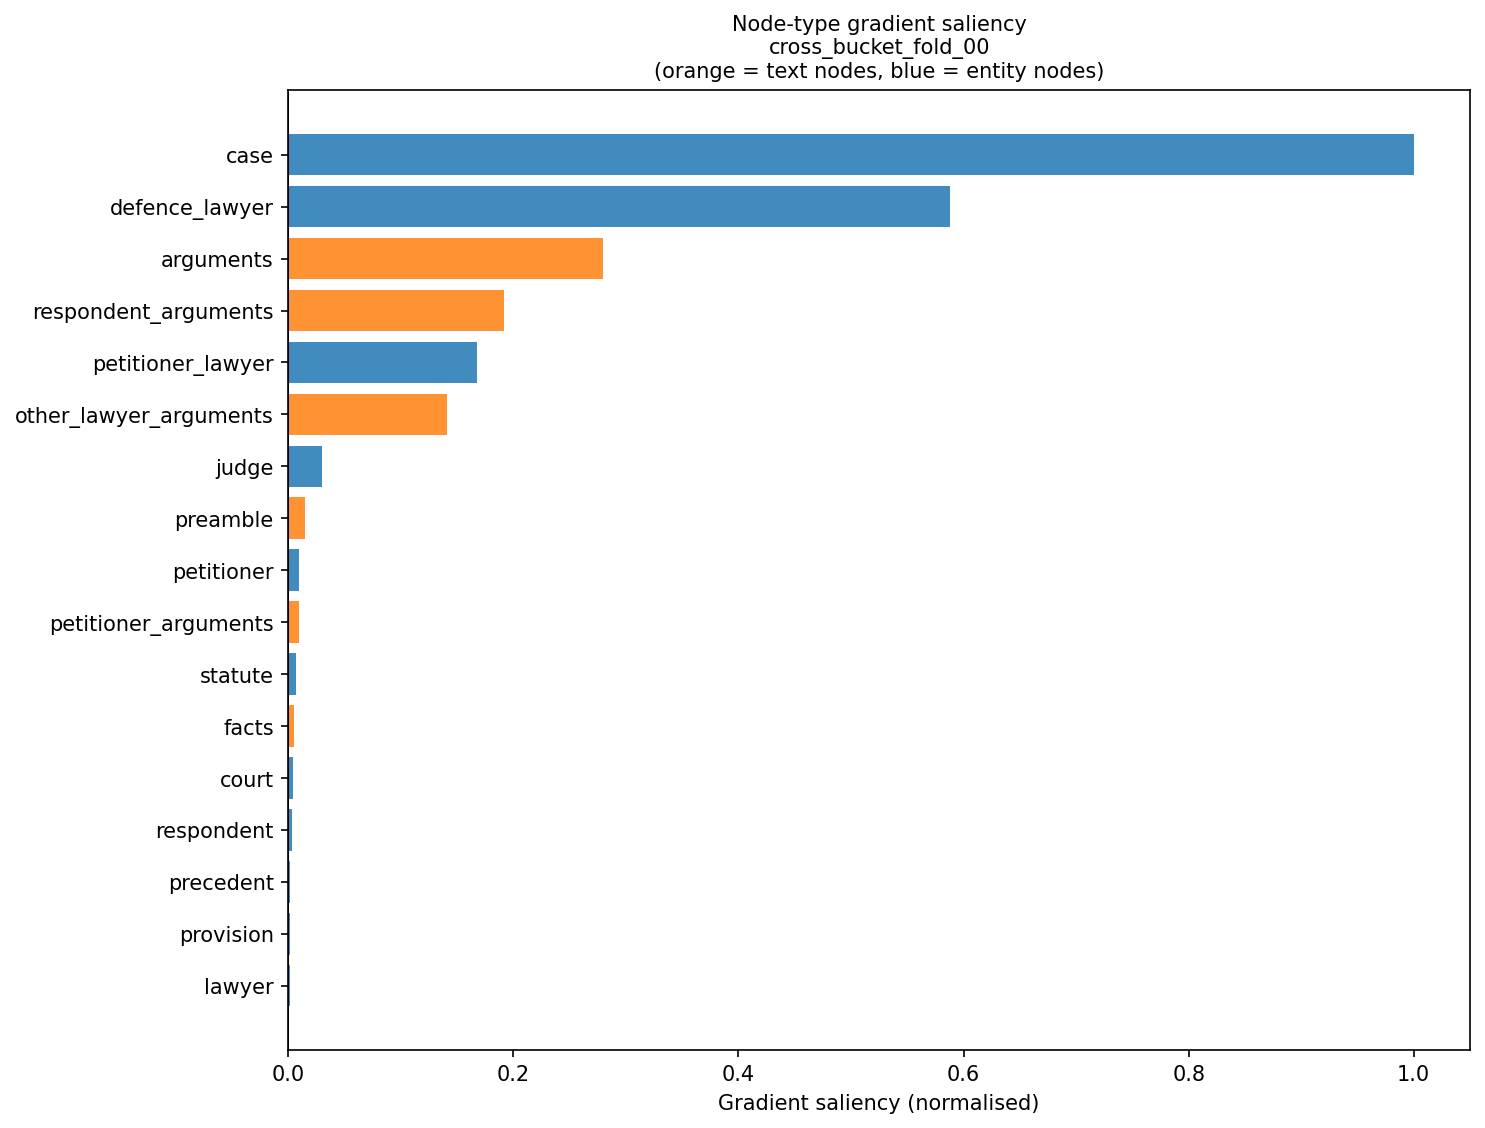
\includegraphics[width=0.65\linewidth]{figures/baseline_cross_bucket_fold00_gradient_saliency.png}
  \caption{{Baseline cross-bucket model (fold~0): node-type
  gradient saliency scores, visualising which node types contribute
  most to the case logit.}}
  \label{fig:attention_saliency_baseline}
\end{figure}

{Figure~\ref{fig:attention_saliency_baseline} makes the
interpretability claims visual. The model is overwhelmingly driven by
the case representation and the argument-bearing text nodes, not by a
single authority type. This helps explain why stripping
names leaves performance almost unchanged: the model's main computation
is structured aggregation of textual legal context into the case node,
not retrieval of identity cues.\par}

\section{SHAP Feature Importance}

Because the post-GNN case embedding is only $64$-dimensional and the
downstream classifier is a logistic regression, a SHAP-style
attribution reduces to the absolute coefficient of each latent
dimension. The top dimensions on the baseline model
(\texttt{dim~45, 21, 52, 20, 38, 25}) each carry the highest mean
absolute SHAP values; the remaining $54$ dimensions contribute smaller,
more distributed weight. No single dimension dominates, which is
evidence that the case embedding is distributed rather than
collapsing onto a small set of predictive features.

\section{Embedding Visualisation (t-SNE)}

t-SNE projections of the pre-GNN and post-GNN case embeddings, coloured
by bucket (\path{tsne_*_by_domain.png}) and by outcome label
(\path{tsne_*_by_label.png}), complete the picture. Three
patterns appear:

\begin{enumerate}
  \item Pre-GNN embeddings cluster strongly by \emph{bucket}: the
    \texttt{bge-m3} representation of the concatenated text already
    separates the five legal domains. Label separability is weak at
    this stage.
  \item Post-GNN embeddings retain the bucket clusters but, within
    each cluster, label-colour separation is visibly improved. The
    HGT's contribution is therefore primarily \emph{within-domain}
    label structure, not between-domain re-organisation.
  \item The \texttt{no\_names} model's t-SNE is qualitatively
    indistinguishable from the baseline's, consistent with the
    probing result and the ablation result: identity information is
    not what the model is using to form the embedding.
\end{enumerate}

\begin{figure}[H]
  \centering
  \begin{minipage}{0.49\textwidth}
    {\footnotesize (a) Baseline pre-GNN, coloured by domain\par}
    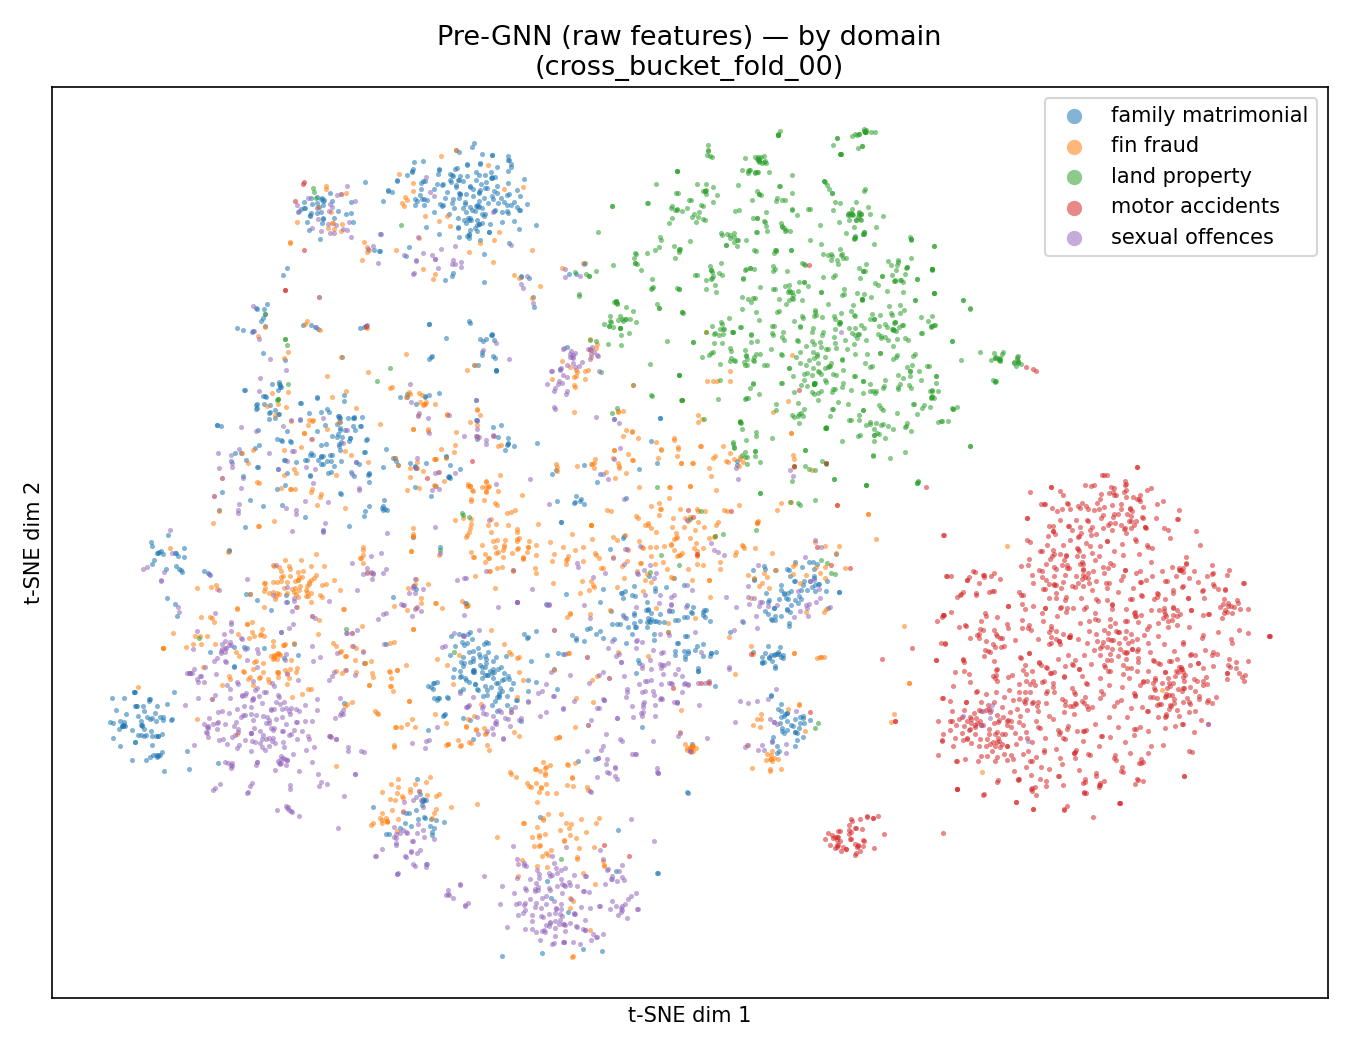
\includegraphics[width=\linewidth]{figures/baseline_cross_bucket_fold00_tsne_pre_by_domain.png}
  \end{minipage}\hfill
  \begin{minipage}{0.49\textwidth}
    {\footnotesize (b) Baseline post-GNN, coloured by domain\par}
    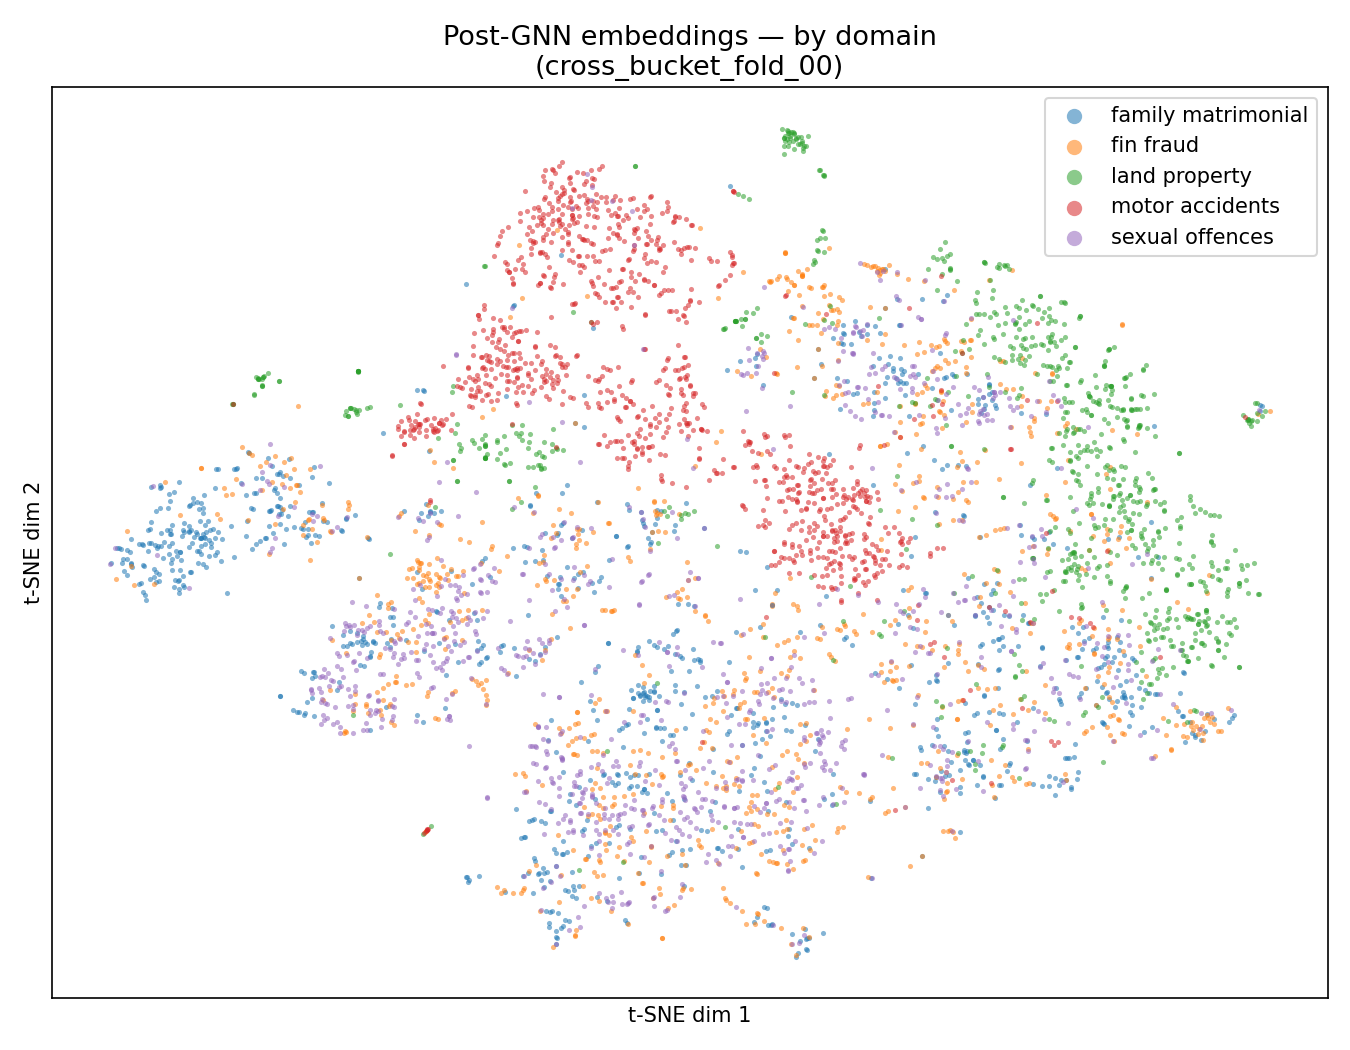
\includegraphics[width=\linewidth]{figures/baseline_cross_bucket_fold00_tsne_post_by_domain.png}
  \end{minipage}

  \vspace{0.5em}

  \begin{minipage}{0.49\textwidth}
    {\footnotesize (c) Baseline pre-GNN, coloured by label\par}
    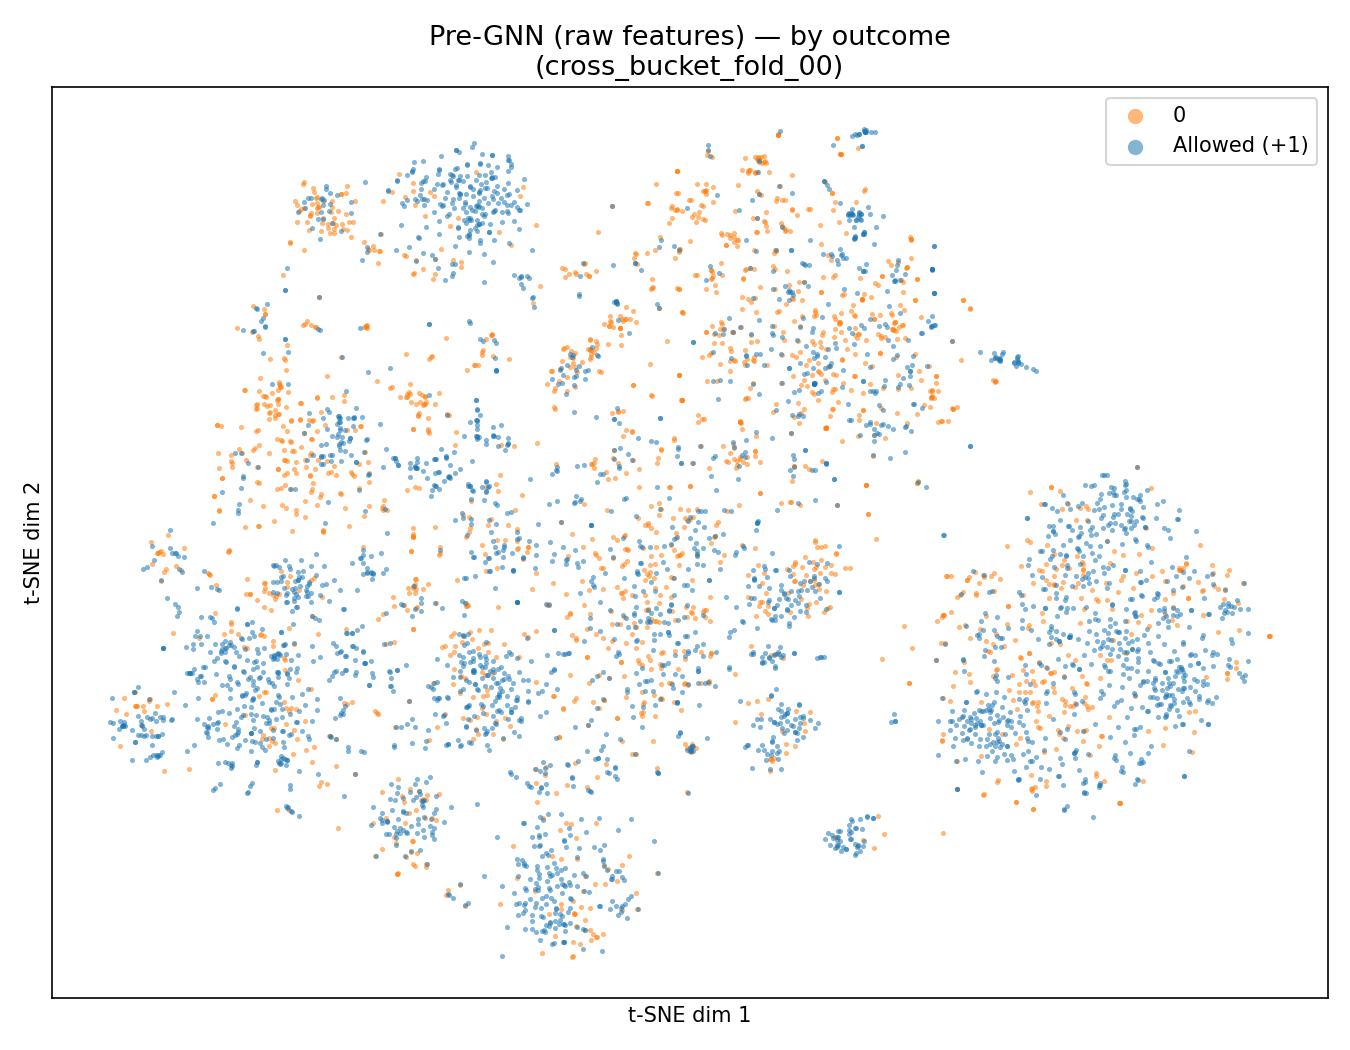
\includegraphics[width=\linewidth]{figures/baseline_cross_bucket_fold00_tsne_pre_by_label.png}
  \end{minipage}\hfill
  \begin{minipage}{0.49\textwidth}
    {\footnotesize (d) Baseline post-GNN, coloured by label\par}
    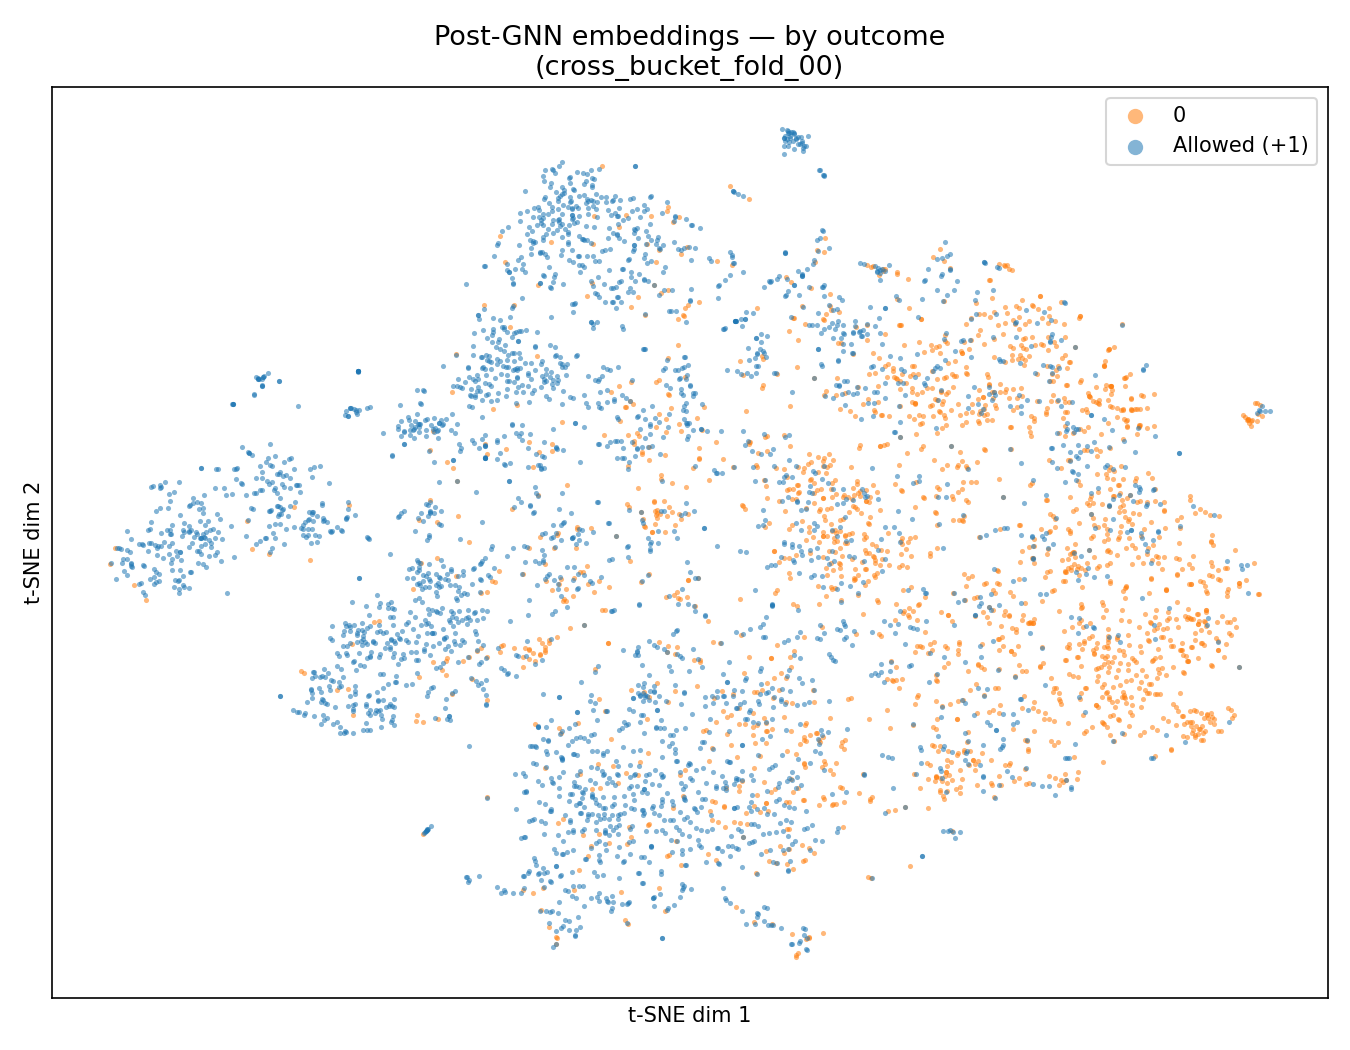
\includegraphics[width=\linewidth]{figures/baseline_cross_bucket_fold00_tsne_post_by_label.png}
  \end{minipage}
  \caption{{Baseline fold-0 t-SNE projections before and
  after graph message passing. The top row tracks domain structure; the
  bottom row tracks outcome structure.}}
  \label{fig:baseline_tsne}
\end{figure}

{Figure~\ref{fig:baseline_tsne} makes the geometry of the
embedding transition easier to read than the summary bullets alone.
Before graph propagation, the representation is already domain-aware:
motor-accidents and land-property form visibly coherent clusters, while
family, fraud, and sexual-offences overlap more heavily. After graph
propagation, these domain regions are preserved, but the label-coloured
view becomes more structured inside them, especially in the larger
motor-accident and land-property regions. This is visually consistent
with the probing result: the GNN is not erasing domain information, but
reorganising each domain locally in a more outcome-informative
way.\par}

\begin{figure}[H]
  \centering
  \begin{minipage}{0.49\textwidth}
    {\footnotesize (a) \texttt{no\_names} pre-GNN, coloured by domain\par}
    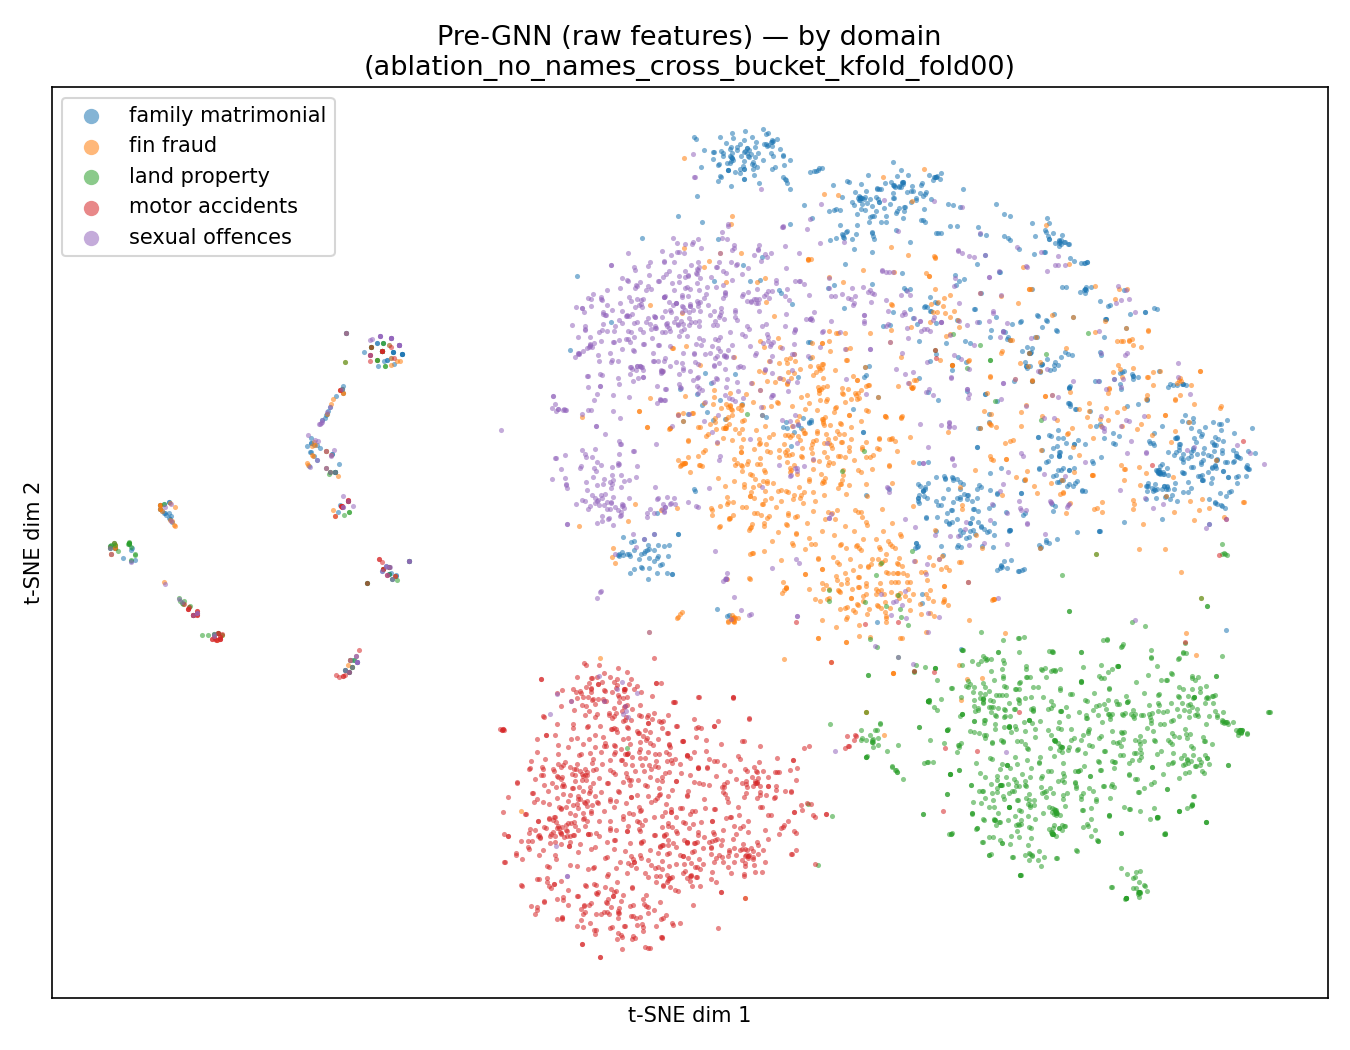
\includegraphics[width=\linewidth]{figures/ablation_no_names_cross_bucket_kfold_fold00_tsne_pre_by_domain.png}
  \end{minipage}\hfill
  \begin{minipage}{0.49\textwidth}
    {\footnotesize (b) \texttt{no\_names} post-GNN, coloured by domain\par}
    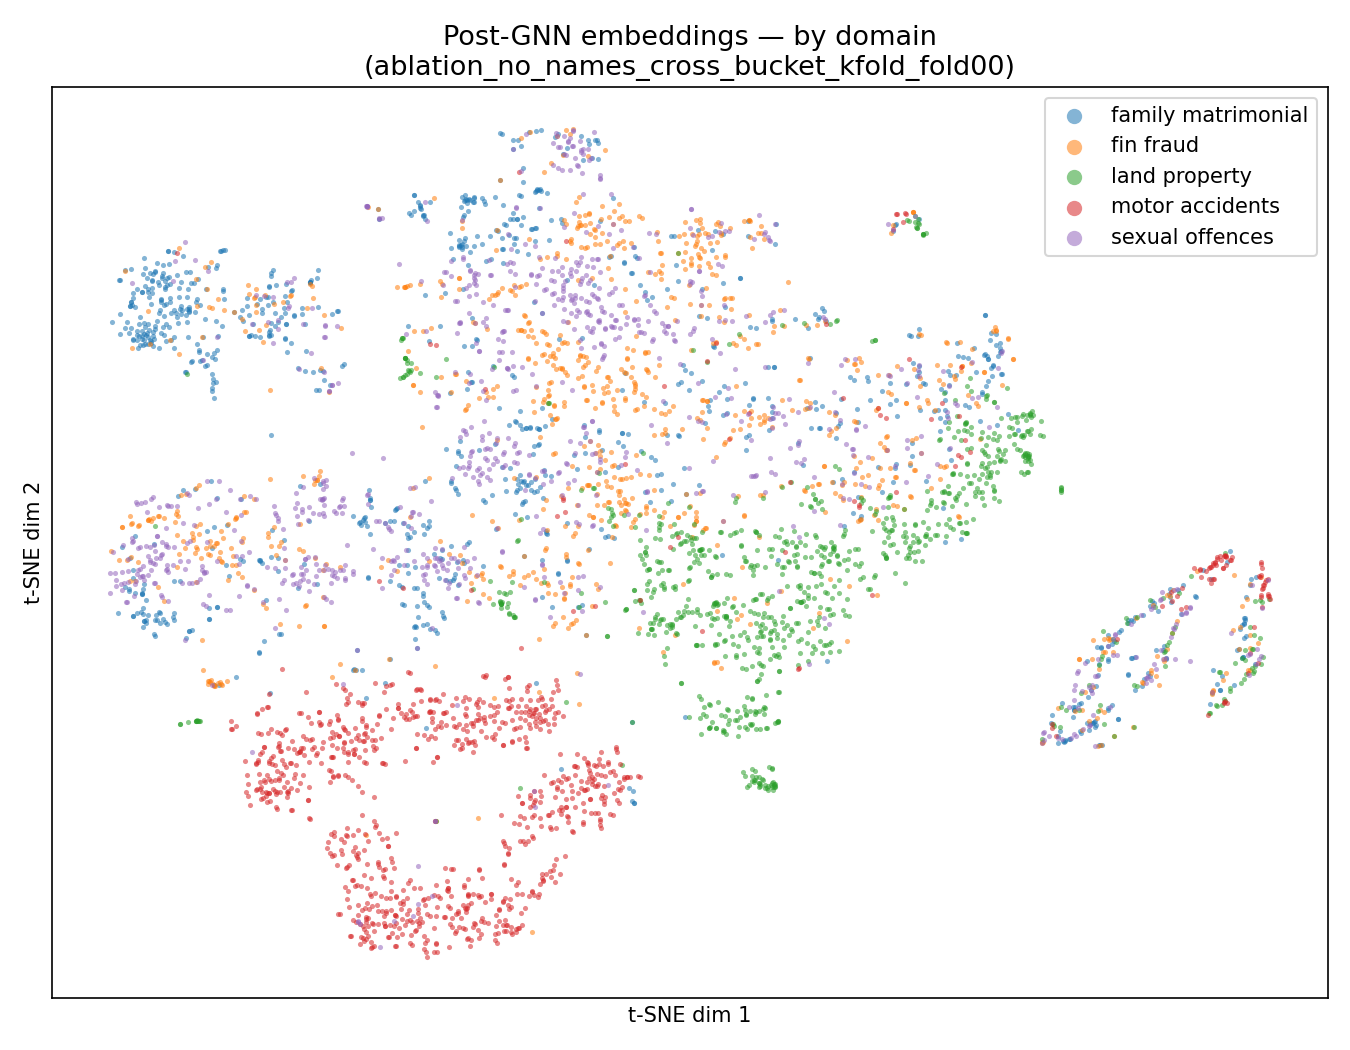
\includegraphics[width=\linewidth]{figures/ablation_no_names_cross_bucket_kfold_fold00_tsne_post_by_domain.png}
  \end{minipage}

  \vspace{0.5em}

  \begin{minipage}{0.49\textwidth}
    {\footnotesize (c) \texttt{no\_names} pre-GNN, coloured by label\par}
    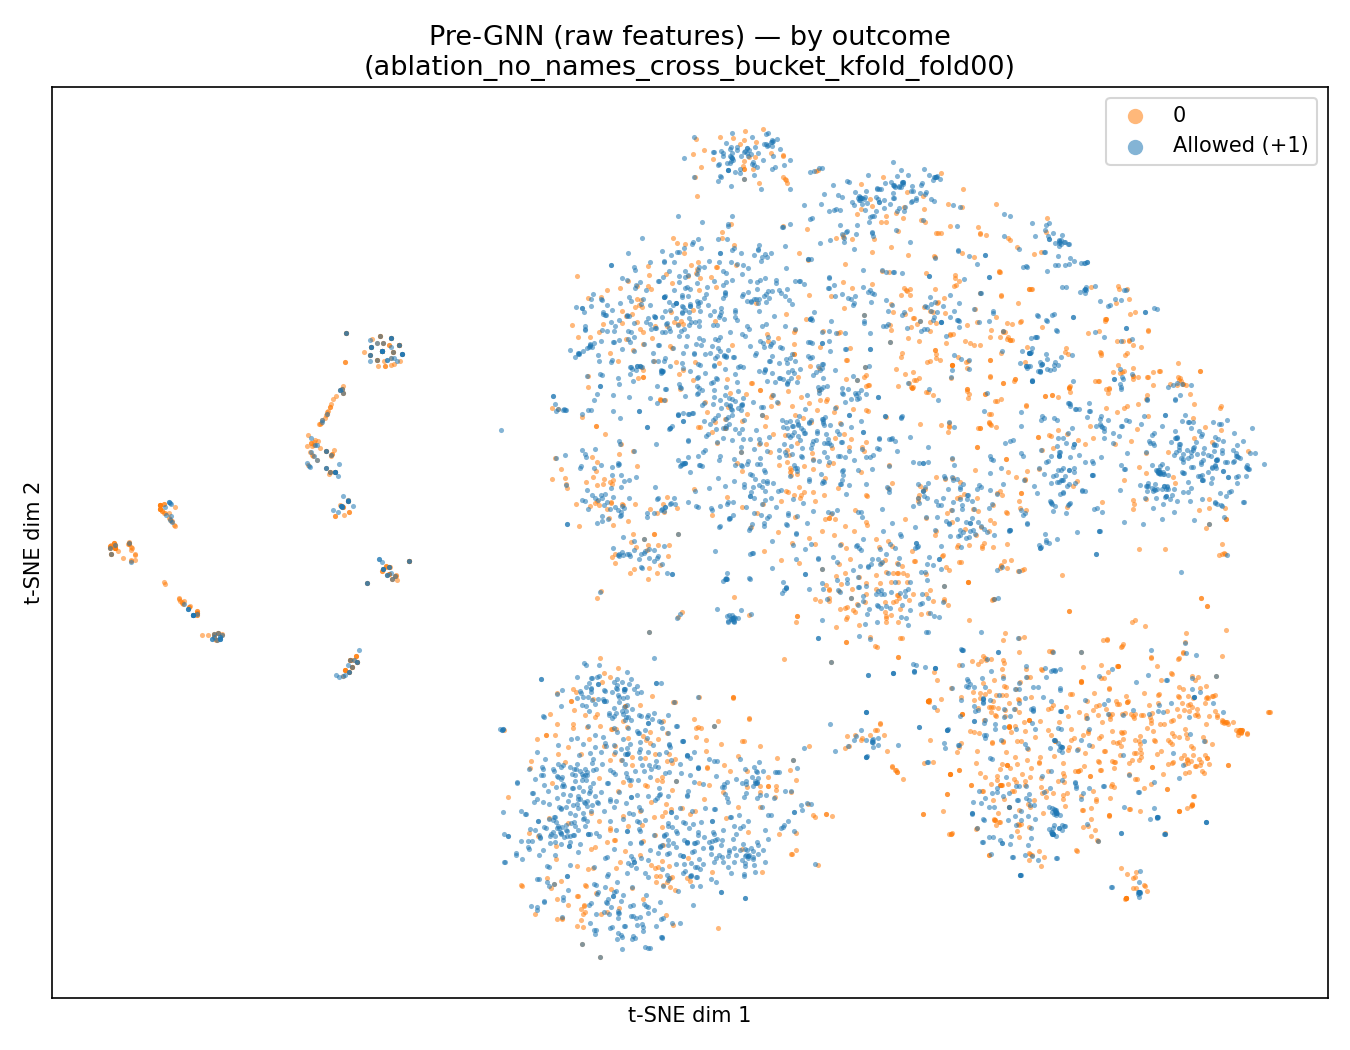
\includegraphics[width=\linewidth]{figures/ablation_no_names_cross_bucket_kfold_fold00_tsne_pre_by_label.png}
  \end{minipage}\hfill
  \begin{minipage}{0.49\textwidth}
    {\footnotesize (d) \texttt{no\_names} post-GNN, coloured by label\par}
    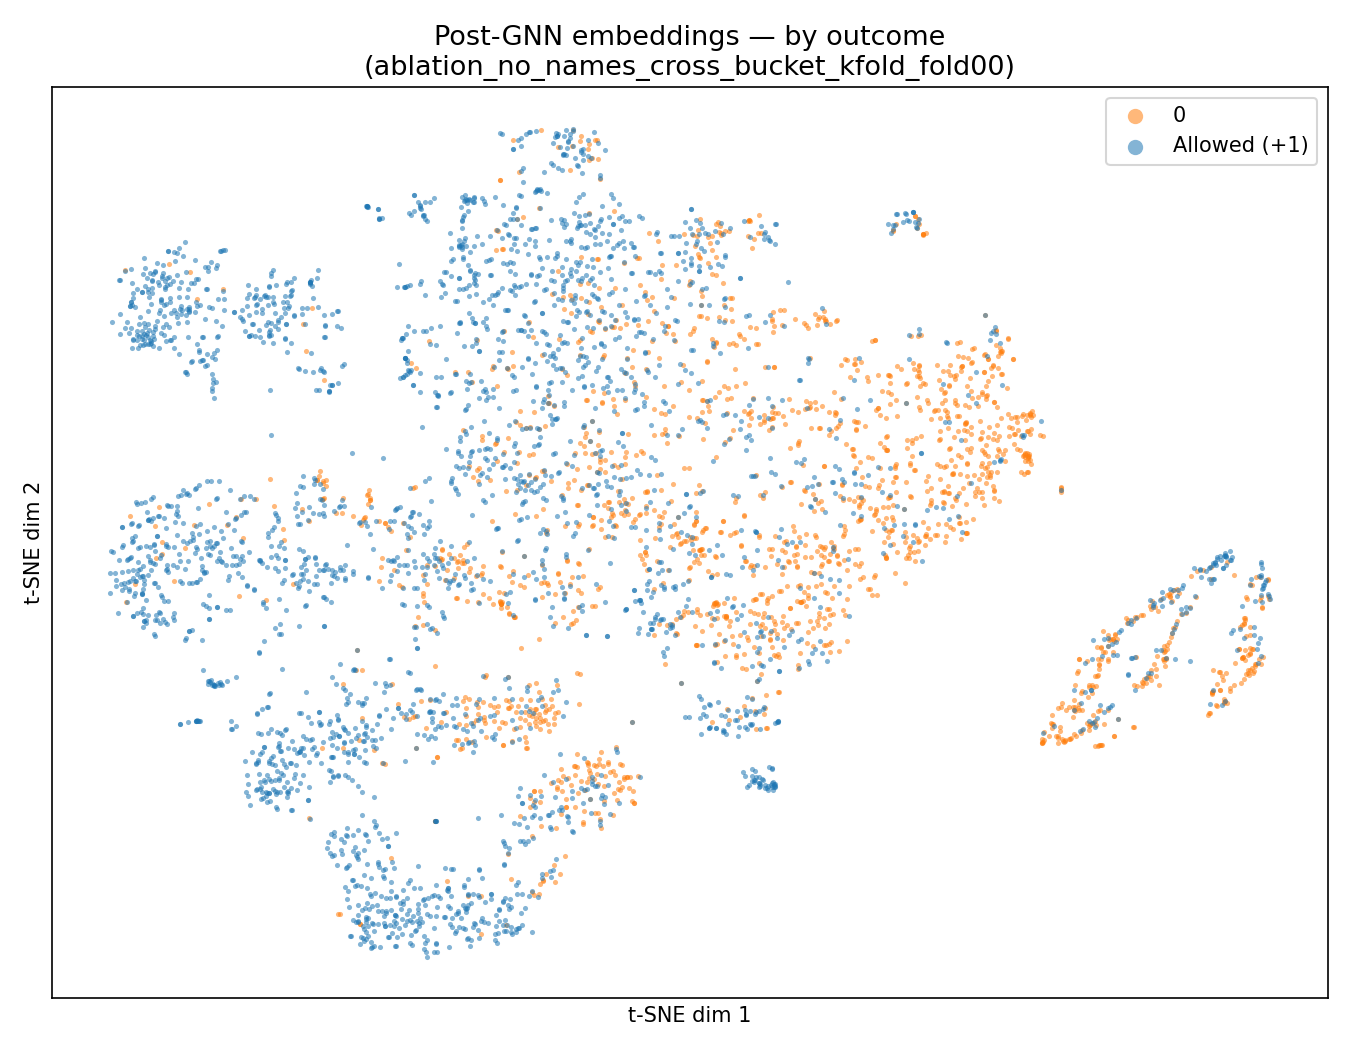
\includegraphics[width=\linewidth]{figures/ablation_no_names_cross_bucket_kfold_fold00_tsne_post_by_label.png}
  \end{minipage}
  \caption{{Corresponding fold-0 t-SNE projections for the
  \texttt{no\_names} ablation.}}
  \label{fig:no_names_tsne}
\end{figure}

{The \texttt{no\_names} t-SNEs in
Figure~\ref{fig:no_names_tsne} reinforce the ablation result from a
different angle. Removing names changes the exact geometry of the
projection, but it does not collapse the domain structure and it does
not remove the post-GNN improvement in label organisation. In other
words, the model still finds a structured outcome space after graph
propagation even when party, lawyer, and judge names are withheld. The
visual similarity is not exact -- t-SNE should not be over-read at that
level -- but the qualitative conclusion is the same as in the accuracy
tables: identity cues are not the dominant organising principle of the
learned case embedding.\par}

\section{Error Analysis}

\noindent\textbf{Error analysis across ablations.} The baseline's
per-domain error pattern (fold~0) -- family-matrimonial $0.825$, fin-fraud
$0.776$, land-property $0.793$, motor-accidents $0.822$,
sexual-offences $0.784$ -- is consistent with the 5-fold mean results
in Table~\ref{tab:per_domain}. The common pattern across every
ablation -- motor-accidents easiest, sexual-offences hardest -- is a
property of the data, not of the model.

\begin{figure}[H]
  \centering
  \begin{minipage}{0.49\textwidth}
    {\footnotesize (a) Baseline accuracy by statute-count bucket\par}
    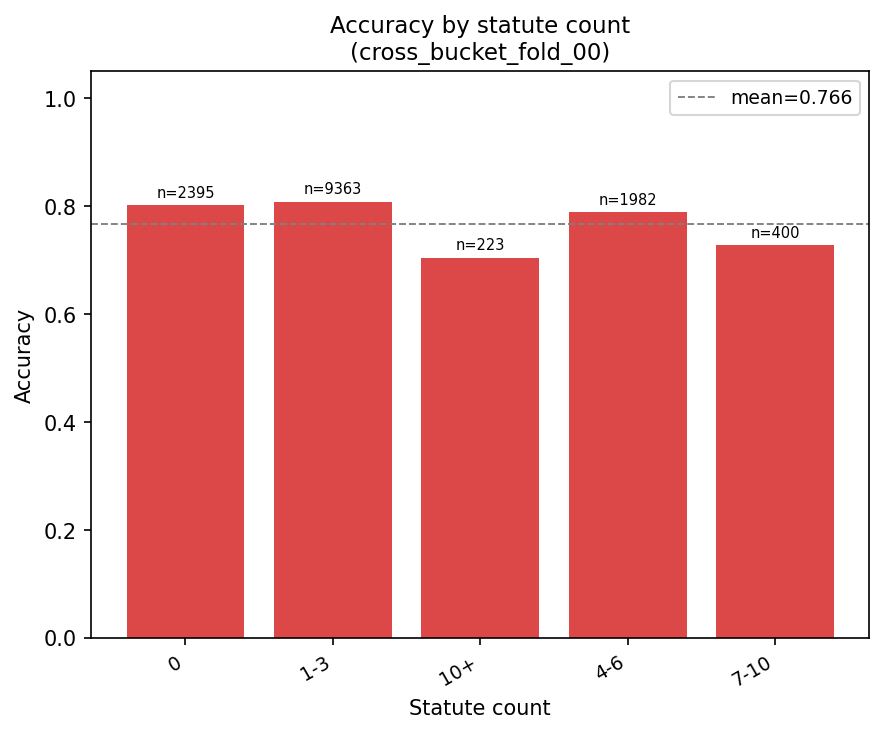
\includegraphics[width=\linewidth]{figures/baseline_cross_bucket_fold00_error_by_statute.png}
  \end{minipage}\hfill
  \begin{minipage}{0.49\textwidth}
    {\footnotesize (b) \texttt{no\_names} accuracy by statute-count bucket\par}
    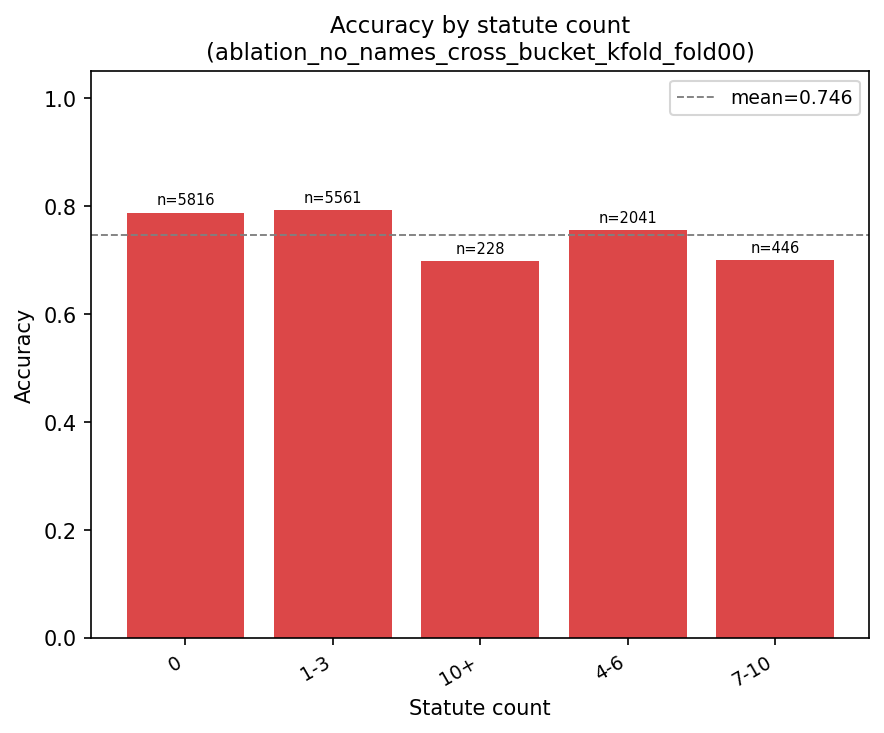
\includegraphics[width=\linewidth]{figures/ablation_no_names_cross_bucket_kfold_fold00_error_by_statute.png}
  \end{minipage}
  \caption{{Held-out fold-0 accuracy as a function of the
  number of statute nodes attached to a case, for the baseline and
  \texttt{no\_names} models.}}
  \label{fig:error_by_statute_count}
\end{figure}

{Figure~\ref{fig:error_by_statute_count} adds an error
pattern that is not visible in the domain-level accuracy tables.
Accuracy is highest when a case cites few statutes and falls once the
authority neighbourhood becomes dense: in the baseline, cases with 0 or
1--3 statute nodes sit near $0.80$ accuracy, while the 7--10 and 10+
buckets are closer to $0.69$--$0.71$. The \texttt{no\_names} model
shows essentially the same curve. This suggests that many of the
residual errors are concentrated in doctrinally crowded cases rather
than in identity-sensitive ones. That is an important distinction: the
hard cases are not those where the model lacks names, but those where
several statutory frames and remedial pathways coexist in the same
judgment.\par}

\begin{figure}[H]
  \centering
  \begin{minipage}{0.49\textwidth}
    {\footnotesize (a) Baseline accuracy by facts-length bucket\par}
    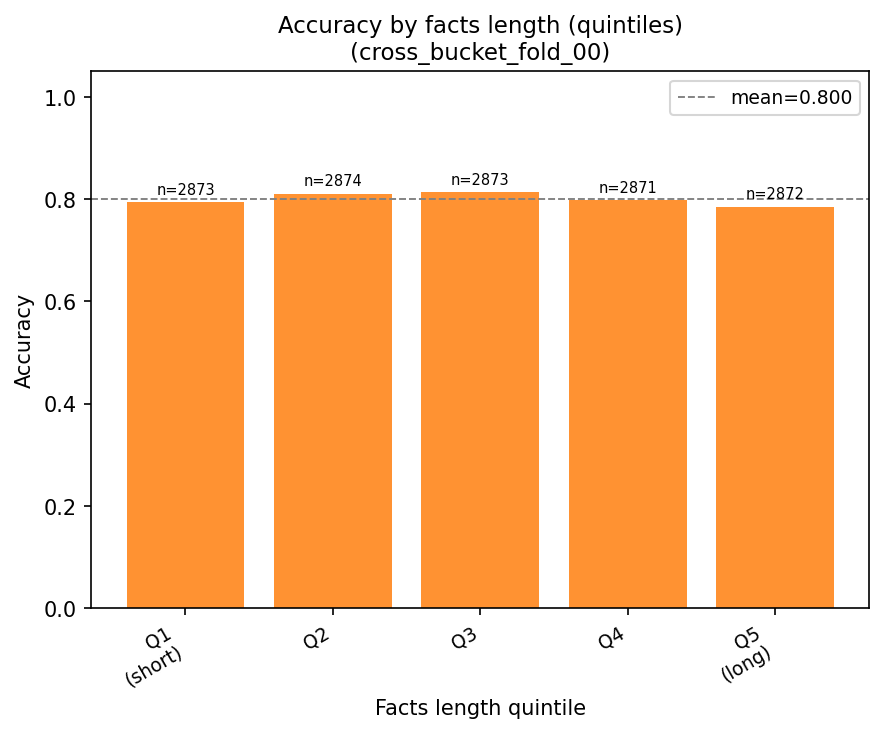
\includegraphics[width=\linewidth]{figures/baseline_cross_bucket_fold00_error_by_facts_len.png}
  \end{minipage}\hfill
  \begin{minipage}{0.49\textwidth}
    {\footnotesize (b) \texttt{no\_names} accuracy by facts-length bucket\par}
    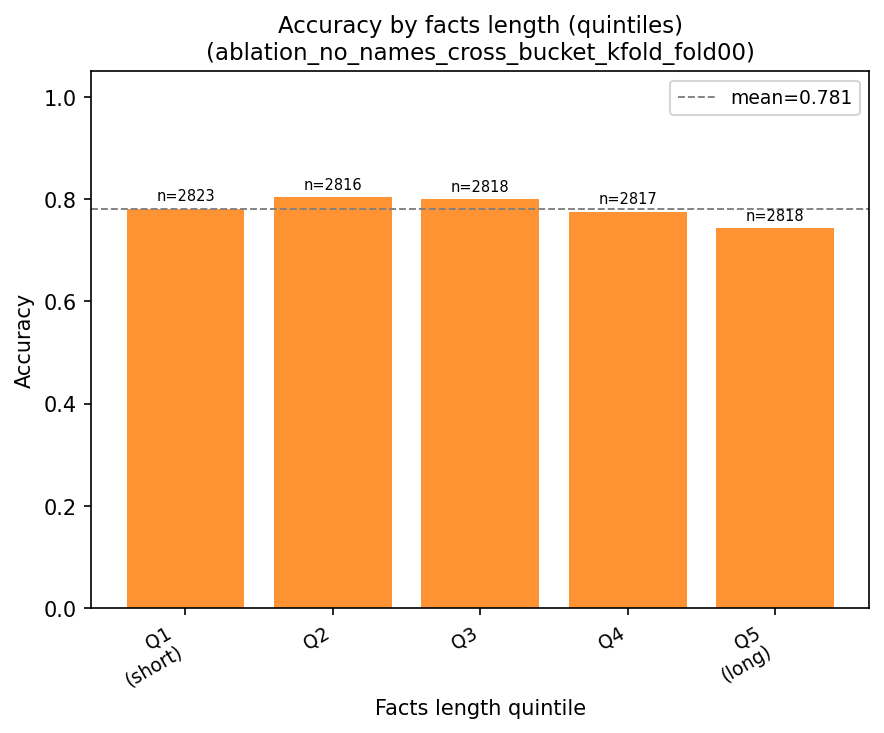
\includegraphics[width=\linewidth]{figures/ablation_no_names_cross_bucket_kfold_fold00_error_by_facts_len.png}
  \end{minipage}
  \caption{{Held-out fold-0 accuracy as a function of the
  length of the facts section, grouped into quintiles from shortest to
  longest, for the baseline and \texttt{no\_names} models.}}
  \label{fig:error_by_facts_length}
\end{figure}

{Figure~\ref{fig:error_by_facts_length} is useful for a
different reason than Figure~\ref{fig:error_by_statute_count}: it tests
whether the remaining errors are concentrated in structurally long
judgments. They are. In the baseline, accuracy falls from about $0.81$
on the shortest-facts quintile to about $0.75$ on the longest-facts
quintile; the \texttt{no\_names} model shows nearly the same decline.
This matters because it links the error analysis back to the ablation
story. The modest, domain-specific gains from
\texttt{hierarchical\_enc} are easier to interpret once the failure
pattern is visible: longer factual narratives do create a harder
representation problem, but the difficulty comes from document
complexity rather than from named entities or party identity.\par}
\fi
